%%%%%%%%%%%
% Preface %
%%%%%%%%%%%
\chapter*{
        %Preface
        前言
        }
     \addcontentsline{toc}{chapter}{
             %Preface
             前言
             }
     \markboth{\sffamily\slshape 
     %Preface
     前言
     }
       {\sffamily\slshape 
       %Preface
       前言
       }

%This text was written to accompany a series of lectures given at the Machine Learning Summer School Buenos Aires, 
% following a lecture series at the Simons Center for Theoretical Computer Science, Berkeley.
%It was extended for the course COS 598D - Optimization for Machine Learning, Princeton University, Spring 2019. 
本书是在布宜诺斯艾利斯举办的机器学习暑期学校的一系列课程,以及在伯克利大学西蒙斯中心举办的理论计算机的一系列课程的讲义。
本讲义随后被扩充为2019年春季普林斯顿大学的机器学习优化课程 COS 598D - Optimization for Machine Learning。

%I am grateful to Paula Gradu for proofreading parts of this manuscript.
%I'm also thankful for the help of the following students and colleagues for corrections and suggestions to this text: 
%Udaya Ghai, John Hallman, No\'{e} Pion, Xinyi Chen. 
%é
我非常感谢 Paula Gradu 对讲义稿件的校对,也非常感谢下列学生和同事对稿件的更正和建议:Udaya Ghai, John Hallman, No\'{e} Pion, Xinyi Chen. 



\begin{figure}[!htb]
        \center{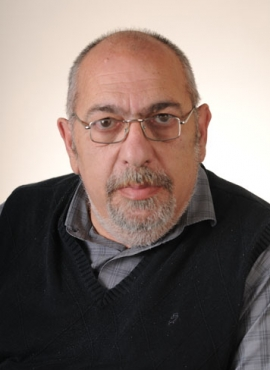
\includegraphics[scale = 1]
        {figs/arkadi.jpg}}
        \caption{\label{fig:my-label}
        %Professor Arkadi Nemirovski, Pioneer of mathematical optimization
        Arkadi Nemirovski 教授, 数学优化的先驱
        }
\end{figure}
    


